\documentclass[11pt,a4paper]{article}

\usepackage[margin=2.3cm]{geometry}
\usepackage{amsmath,amssymb}
\usepackage{graphicx}
\usepackage{tikz}
\usetikzlibrary{arrows.meta,calc,shapes.geometric,backgrounds}
\usepackage{booktabs}
\usepackage{siunitx}
\usepackage{xcolor}
\usepackage{listings}
\usepackage{hyperref}
\usepackage{caption}
\usepackage{enumitem}

\hypersetup{colorlinks=true,linkcolor=blue!50!black,citecolor=blue!50!black,urlcolor=blue!50!black}
\graphicspath{{../results/}}

\lstset{basicstyle=\ttfamily\small,keywordstyle=\color{blue!60!black}\bfseries,
        commentstyle=\color{gray},frame=single,breaklines=true,columns=fixed,keepspaces=true,basewidth=0.5em}

\title{\textbf{Approximate Multiply--Accumulate Units for\\Energy-Efficient DNN Accelerators}\\[4pt]
       \large Error Characterization and Application-Level Evaluation}
\author{Sina Mozaffari Rad \and Fatemeh Dastyafteh\\[4pt]
        \small Co-developed project\quad\textbar\quad
        \url{https://github.com/GitCodingMates/approx-mac-dnn}}
\date{November 2026}

\begin{document}
\maketitle

\begin{abstract}
Multiply--accumulate (MAC) operations dominate both the computation and the
energy budget of deep neural network (DNN) inference. Because DNNs are
inherently tolerant to small numerical errors, the exact multiplier inside each
MAC can be replaced with a cheaper \emph{approximate} multiplier. This project
studies that trade-off for 8-bit signed arithmetic. Bit-accurate models of an
exact array multiplier, three column-truncated multipliers, and Mitchell's
logarithmic multiplier were developed and characterized exhaustively over all
$2^{16}$ input pairs. A fully-connected network was trained on MNIST,
quantized to int8 with int32 accumulation, and evaluated with every
multiplication routed through each approximate design. Results show that even
a multiplier with a mean relative error of \SI{23.9}{\percent} reduces
classification accuracy by only \SI{0.42}{\percent}. All designs were
implemented in Verilog, verified exhaustively against the reference models,
and synthesized with Yosys. The truncated multiplier reduces multiplier area by
\SI{59.8}{\percent} and complete MAC area by \SI{38.9}{\percent}, whereas
the logarithmic multiplier saves less than \SI{5}{\percent} at this operand
width, showing that the best approximation strategy depends on the datapath
width and cannot be chosen from error metrics alone.
\end{abstract}

\section{Introduction}
The processing elements (PEs) of a DNN accelerator are, at their core, MAC
units. In an 8-bit datapath the multiplier is the largest and most
power-hungry part of the PE, so its cost scales directly with the size of the
PE array. \emph{Approximate computing} exploits the error resilience of
DNNs: errors in individual products are partially averaged out across long dot
products, and the final classification decision (an \texttt{argmax}) is
insensitive to small perturbations of the output scores.

The goals of this project are:
\begin{enumerate}[nosep]
  \item to build bit-accurate, hardware-oriented models of representative
        approximate multipliers;
  \item to characterize their arithmetic error with standard metrics;
  \item to measure their impact on the accuracy of a quantized neural network;
  \item to implement them in synthesizable Verilog and verify the RTL
        exhaustively against the reference models;
  \item to quantify the hardware savings by logic synthesis and identify
        the best area--accuracy trade-offs (Section~\ref{sec:synth}).
\end{enumerate}

\section{Multiplier Designs}
All designs operate on 8-bit two's-complement operands
$a,b\in[-128,127]$ and are implemented in sign-magnitude form: the magnitudes
$|a|,|b|\in[0,128]$ are multiplied and the sign is restored as
$\operatorname{sgn}(a)\oplus\operatorname{sgn}(b)$. This makes the error of
every approximate design symmetric around zero.

\subsection{Exact array multiplier (baseline)}
The product is the sum of $N^2$ partial-product bits,
\begin{equation}
  P = \sum_{i=0}^{N-1}\sum_{j=0}^{N-1} a_i\, b_j\, 2^{i+j}, \qquad N = 8 .
\end{equation}

\subsection{Column-truncated multiplier}
All partial-product bits whose weight falls below column $k$ are removed:
\begin{equation}
  P_{\text{trunc}}(k) = \sum_{i+j\ \ge\ k} a_i\, b_j\, 2^{i+j}.
\end{equation}
Each removed bit eliminates one AND gate and its share of the
carry-save adder tree. For $k=4,6,8$, respectively 10, 21 and 36 of the 64
partial-product bits are removed. No error-compensation constant is added, so
the design always under-estimates the product magnitude.

\subsection{Mitchell logarithmic multiplier}
Writing each operand as $x = 2^{k}(1+f)$, where $k=\lfloor\log_2 x\rfloor$ is
found by a leading-one detector (LOD) and $0\le f<1$, Mitchell's
algorithm~\cite{mitchell1962} approximates
$\log_2(ab)\approx k_1+k_2+f_1+f_2$. With $x_i = |a_i| - 2^{k_i}$, an
exact-integer form suitable for hardware is
\begin{equation}
  S = x_1 2^{k_2} + x_2 2^{k_1},\qquad
  P_{\text{Mitchell}} =
  \begin{cases}
    2^{k_1+k_2} + S, & S < 2^{k_1+k_2}\\
    2S,              & \text{otherwise.}
  \end{cases}
\end{equation}
The datapath therefore consists only of two LODs, barrel shifters and a
single adder; no partial-product array is required.

\paragraph{Error bound.} The bound below was derived by
Mitchell~\cite{mitchell1962}; it is restated here in the
notation of Eq.~(3). Since $x_i = 2^{k_i} f_i$, we have
$S = 2^{k_1+k_2}(f_1+f_2)$, while the exact product is
$P = 2^{k_1+k_2}(1+f_1)(1+f_2)$. Two cases follow.

\emph{Case $f_1+f_2<1$.} Here $P_{\text{Mitchell}} = 2^{k_1+k_2}(1+f_1+f_2)$
and
\begin{equation}
  \frac{P-P_{\text{Mitchell}}}{P} = \frac{f_1 f_2}{(1+f_1)(1+f_2)} \;\ge 0 .
\end{equation}

\emph{Case $f_1+f_2\ge 1$.} Here $P_{\text{Mitchell}} = 2^{k_1+k_2+1}(f_1+f_2)$
and
\begin{equation}
  \frac{P-P_{\text{Mitchell}}}{P} = \frac{(1-f_1)(1-f_2)}{(1+f_1)(1+f_2)} \;\ge 0 .
\end{equation}

Both expressions are non-negative, so the multiplier never over-estimates.
In the first case, write $g(f)=f/(1+f)$, which is increasing; the error is
$g(f_1)g(f_2)$ and grows with both fractions, so its supremum lies on the
boundary $f_1+f_2=1$. In the second case, $h(f)=(1-f)/(1+f)$ is decreasing
and the error $h(f_1)h(f_2)$ is also largest on $f_1+f_2=1$. On that line,
with $f_2 = 1-f_1$, both cases give the same value,
\begin{equation}
  E(f_1) = \frac{f_1(1-f_1)}{(1+f_1)(2-f_1)} ,
\end{equation}
which is symmetric about $f_1=\tfrac12$. Setting $E'(f_1)=0$ gives
$(1-2f_1)\bigl[(1+f_1)(2-f_1)-f_1(1-f_1)\bigr]=0$, where the bracket equals 2,
so $f_1=f_2=\tfrac12$ and
\begin{equation}
  E_{\max} = \frac{\tfrac12\cdot\tfrac12}{\tfrac32\cdot\tfrac32}
           = \frac{1}{9} \approx \SI{11.1}{\percent}.
\end{equation}
This is the well-known worst-case relative error of the Mitchell
multiplier~\cite{mitchell1962,jiang2020survey}. For 8-bit operands
$f=\tfrac12$ is reachable, e.g.\ $a=b=3$ gives $P=9$ and
$P_{\text{Mitchell}}=8$. The exhaustive evaluation of the bit-accurate model
over all operand pairs (Section~\ref{sec:results}) confirms a maximum
relative error of exactly $1/9$, attained whenever $|a|=3\cdot 2^{i}$ and
$|b|=3\cdot 2^{j}$.

\section{Methodology}

\subsection{Bit-accurate reference models}
Each design is described in Python/NumPy at the bit level
(\texttt{python/approx\_mult.py}), mirroring the intended RTL structure
(partial-product selection, LOD, shifts). These models serve as the golden
reference for RTL verification. For fast evaluation, each model is expanded
into a $256\times256$ product look-up table.

\subsection{Error metrics}
Every design is evaluated over all $65{,}536$ input pairs. With
$P$ the exact and $\hat P$ the approximate product, and
$\text{ED}=|\hat P - P|$, the following metrics are reported~\cite{jiang2020survey}:
\begin{itemize}[nosep]
  \item \textbf{ER} -- error rate, fraction of inputs with $\text{ED}\neq 0$;
  \item \textbf{MED} -- mean error distance, $\mathbb{E}[\text{ED}]$;
  \item \textbf{NMED} -- MED normalized by the maximum product ($128^2$);
  \item \textbf{MRED} -- mean relative error distance, $\mathbb{E}[\text{ED}/|P|]$ over $P\neq0$;
  \item \textbf{Max ED} -- worst-case absolute error.
\end{itemize}

\subsection{Quantized neural network}
A 784--128--10 multilayer perceptron with ReLU activation was trained on
MNIST~\cite{lecun1998} for eight epochs using mini-batch SGD
(batch 128, learning rate 0.1), implemented directly in NumPy.
The trained network was then quantized following the integer-only inference
scheme of~\cite{jacob2018}:
\begin{itemize}[nosep]
  \item inputs: $x_q = \operatorname{round}(127\,x)$, $x\in[0,1]$;
  \item weights: symmetric per-tensor int8, $s_w = \max|W|/127$;
  \item biases: int32 at scale $s_x s_w$;
  \item accumulation: int32;
  \item hidden activations: requantized to unsigned 7-bit values using a scale
        calibrated on 5{,}000 training images (99.99th percentile).
\end{itemize}
During approximate inference, \emph{every} multiplication in both layers is
replaced by the corresponding approximate multiplier, exactly as it would
occur inside the accelerator's PEs. Accuracy is measured on the full
10{,}000-image test set.

\section{Results}\label{sec:results}

\subsection{Arithmetic error}
Table~\ref{tab:error} summarizes the exhaustive error characterization, and
Figure~\ref{fig:heat} shows how the relative error is distributed over the
input space.

\begin{table}[h]
\centering
\caption{Error characterization over all $2^{16}$ signed 8-bit input pairs.}
\label{tab:error}
\begin{tabular}{lrrrrr}
\toprule
Multiplier & ER (\%) & MED & NMED (\%) & MRED (\%) & Max ED \\
\midrule
Exact          & 0.00  & 0.00   & 0.000 & 0.00  & 0    \\
Truncated $k{=}4$ & 81.25 & 12.25  & 0.075 & 1.72  & 49   \\
Truncated $k{=}6$ & 93.75 & 80.25  & 0.490 & 7.59  & 321  \\
Truncated $k{=}8$ & 98.05 & 384.75 & 2.348 & 23.87 & 1537 \\
Mitchell       & 87.89 & 151.34 & 0.924 & 3.70  & 1024 \\
\bottomrule
\end{tabular}
\end{table}

\begin{figure}[h]
\centering
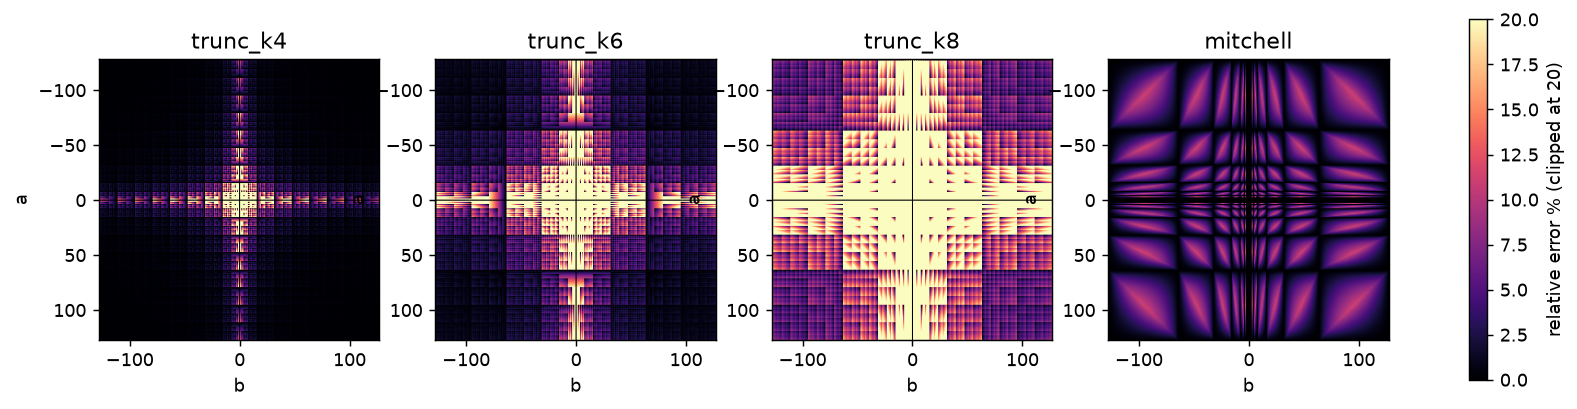
\includegraphics[width=\textwidth]{error_heatmaps.png}
\caption{Relative error (\%) of each approximate multiplier as a function of
its operands. Truncation errors concentrate at small operands, where the
removed low-order columns carry a larger share of the product; Mitchell's
error depends on the fractional parts of both operands and is bounded at
about \SI{11}{\percent}.}
\label{fig:heat}
\end{figure}

The measured MRED of the Mitchell multiplier (\SI{3.70}{\percent}) agrees with
the value reported in the literature (\SI{\approx3.8}{\percent}), which
validates the model. Truncation exhibits a clear knob: each increase of $k$ by
two columns raises the MED by roughly a factor of five.

\subsection{Application-level accuracy}
\begin{table}[h]
\centering
\caption{MNIST test accuracy of the int8 MLP with each multiplier.
Float32 reference: \SI{96.82}{\percent}.}
\label{tab:acc}
\begin{tabular}{lrr}
\toprule
Multiplier & Accuracy (\%) & $\Delta$ vs.\ exact int8 \\
\midrule
Exact (int8)      & 96.81 & --    \\
Truncated $k{=}4$ & 96.82 & $+0.01$ \\
Truncated $k{=}6$ & 96.77 & $-0.04$ \\
Truncated $k{=}8$ & 96.39 & $-0.42$ \\
Mitchell          & 96.77 & $-0.04$ \\
\bottomrule
\end{tabular}
\end{table}

Table~\ref{tab:acc} shows the central result of this project: arithmetic error
and application error are only weakly coupled. Int8 quantization itself costs
just \SI{0.01}{\percent}. Truncation up to $k=6$ and the Mitchell multiplier are
practically lossless, and even $k=8$ truncation---which removes more than half
of the partial-product array and has an MRED above \SI{20}{\percent}---loses
less than half a percentage point. Two effects explain this resilience:
\begin{enumerate}[nosep]
  \item \textbf{Error averaging.} Each output neuron accumulates up to 784
        products; independent errors partially cancel, so the relative error
        of the sum is far smaller than that of a single product.
  \item \textbf{Decision robustness.} Classification depends only on the
        ranking of the output scores, so a systematic, roughly proportional
        under-estimation (as produced by both truncation and Mitchell) rarely
        changes the \texttt{argmax}.
\end{enumerate}

\section{RTL Implementation}
All designs are written in synthesizable Verilog-2001 (\texttt{rtl/}) and
share a common \texttt{sign\_mag} front end that converts the
two's-complement operands to 8-bit magnitudes and computes the product sign.

\begin{itemize}[nosep]
  \item \texttt{mul\_exact} -- baseline $8\times8$ magnitude multiplier.
  \item \texttt{mul\_trunc \#(K)} -- the partial-product array is built
        row by row; in row $j$ the bits of $|a|$ below position $K-j$ are
        masked with an elaboration-time constant, so the corresponding AND
        gates and adder inputs are removed by synthesis rather than gated at
        run time. A single parameter covers the whole design space.
  \item \texttt{mul\_mitchell} -- two priority-encoder LODs, mantissa
        extraction by clearing the leading one, two barrel shifters, one
        16-bit adder and a comparator/multiplexer that selects between the
        two cases of Eq.~(3).
  \item \texttt{mac \#(MUL,K)} -- a two-stage pipelined MAC. Stage~1
        registers the product, stage~2 sign-extends it and accumulates into
        a 32-bit register. A \texttt{clr} input restarts the accumulation so
        consecutive dot products can be streamed without bubbles, and an
        \texttt{en} input supports idle cycles. The multiplier is selected at
        elaboration time with a \texttt{generate} block, so all variants share
        one PE description.
\end{itemize}

\begin{figure}[t]
\centering
\resizebox{\textwidth}{!}{% Block diagram of the pipelined MAC unit (rtl/mac.v).
% Requires: tikz with libraries arrows.meta, backgrounds
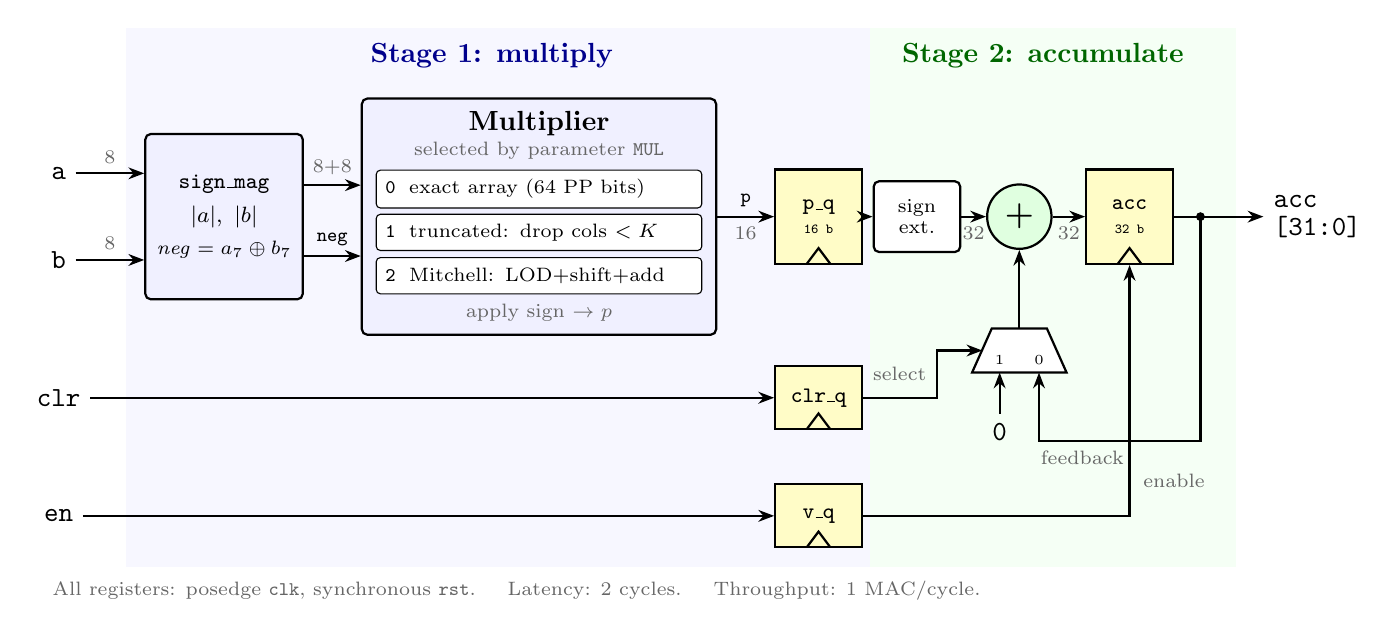
\begin{tikzpicture}[
    font=\footnotesize,
    >={Stealth[length=2mm]},
    wire/.style={thick, ->},
    blk/.style={draw, thick, rounded corners=2pt, fill=blue!6, align=center},
    sub/.style={draw, rounded corners=1.5pt, fill=white, text width=3.9cm,
                minimum height=0.46cm, font=\scriptsize, anchor=center},
    reg/.style={draw, thick, fill=yellow!22, minimum width=1.1cm, minimum height=1.2cm,
                align=center, font=\footnotesize\ttfamily,
                path picture={\draw ([xshift=-1.5mm]path picture bounding box.south)
                              -- ++(1.5mm,2mm) -- ++(1.5mm,-2mm);}},
    note/.style={font=\scriptsize, text=black!60},
]

% ---------------------------------------------------------------- stages
\begin{scope}[on background layer]
  \fill[blue!3]  (1.05,-1.55) rectangle (10.5,5.3);
  \fill[green!4] (10.5,-1.55) rectangle (15.15,5.3);
\end{scope}
\node[font=\bfseries, text=blue!55!black]  at (5.7,4.95)  {Stage 1: multiply};
\node[font=\bfseries, text=green!40!black] at (12.7,4.95) {Stage 2: accumulate};

% ---------------------------------------------------------------- datapath
\node[blk, minimum width=2.0cm, minimum height=2.1cm] (sm) at (2.3,2.9)
     {\texttt{\textbf{sign\_mag}}\\[3pt] $|a|,\ |b|$\\[2pt]
      \scriptsize $\mathit{neg}=a_7\oplus b_7$};

\node[blk, minimum width=4.5cm, minimum height=3.0cm] (mul) at (6.3,2.9) {};
\node[font=\bfseries] at (6.3,4.08) {Multiplier};
\node[note] at (6.3,3.74) {selected by parameter \texttt{MUL}};
\node[sub] at (6.3,3.25) {\texttt{\textbf{0}}\; exact array (64 PP bits)};
\node[sub] at (6.3,2.70) {\texttt{\textbf{1}}\; truncated: drop cols $<K$};
\node[sub] at (6.3,2.15) {\texttt{\textbf{2}}\; Mitchell: LOD+shift+add};
\node[note] at (6.3,1.68) {apply sign $\rightarrow p$};

\node[reg] (pq) at (9.85,2.9) {p\_q\\[-1pt]\tiny 16 b};
\node[blk, fill=white, minimum width=1.1cm, minimum height=0.9cm] (sx) at (11.1,2.9)
     {\scriptsize sign\\[-2pt]\scriptsize ext.};
\node[draw, thick, circle, fill=green!12, minimum size=0.75cm, font=\large\bfseries]
     (add) at (12.4,2.9) {+};
\node[reg] (acc) at (13.8,2.9) {acc\\[-1pt]\tiny 32 b};

% inputs
\node[font=\ttfamily\bfseries] (a) at (0.2,3.45) {a};
\node[font=\ttfamily\bfseries] (b) at (0.2,2.35) {b};
\draw[wire] (a) -- (a -| sm.west) node[pos=.5, above, note] {8};
\draw[wire] (b) -- (b -| sm.west) node[pos=.5, above, note] {8};

% stage 1 wires
\draw[wire] ([yshift=4mm]sm.east) -- ([yshift=4mm]sm.east -| mul.west)
     node[pos=.5, above, note] {8+8};
\draw[wire] ([yshift=-5mm]sm.east) -- ([yshift=-5mm]sm.east -| mul.west)
     node[pos=.5, above, font=\scriptsize\ttfamily] {neg};
\draw[wire] (mul.east |- pq) -- (pq.west)
     node[pos=.5, above, font=\scriptsize\ttfamily] {p}
     node[pos=.5, below, note] {16};

% stage 2 wires
\draw[wire] (pq.east) -- (sx.west);
\draw[wire] (sx.east) -- (add.west) node[pos=.5, below, note] {32};
\draw[wire] (add.east) -- (acc.west) node[pos=.5, below, note] {32};
\draw[wire] (acc.east) -- (15.5,2.9)
     node[right, font=\ttfamily\bfseries, align=left] {acc\\[-2pt][31:0]};

% clear multiplexer and feedback
\draw[thick, fill=white] (11.8,0.92) -- (13.0,0.92) -- (12.75,1.48) -- (12.05,1.48) -- cycle;
\coordinate (muxN) at (12.4,1.48);
\coordinate (muxW) at (11.93,1.2);
\draw[wire] (muxN) -- (add.south);
\coordinate (fb) at (14.7,2.9);
\fill (fb) circle (1.6pt);
\draw[wire] (fb) |- (12.65,0.05) -- (12.65,0.92);
\draw[wire] (12.15,0.4) node[below, font=\ttfamily] {0} -- (12.15,0.92);
\node[font=\tiny] at (12.15,1.08) {1};
\node[font=\tiny] at (12.65,1.08) {0};
\node[note, anchor=north] at (13.2,0.05) {feedback};

% ---------------------------------------------------------------- control
\node[font=\ttfamily\bfseries] (clr) at (0.2,0.6)  {clr};
\node[font=\ttfamily\bfseries] (en)  at (0.2,-0.9) {en};
\node[reg, minimum height=0.8cm] (cq) at (9.85,0.6)  {clr\_q};
\node[reg, minimum height=0.8cm] (vq) at (9.85,-0.9) {v\_q};
\draw[wire] (clr) -- (cq.west);
\draw[wire] (en)  -- (vq.west);
\draw[wire] (cq.east) -- (11.35,0.6) |- (muxW)
     node[pos=.25, left, note] {select};
\draw[wire] (vq.east) -| (acc.south);
\node[note, anchor=west] at (13.85,-0.45) {enable};

% ---------------------------------------------------------------- footer
\node[note, anchor=west] at (0.0,-1.85)
     {All registers: posedge \texttt{clk}, synchronous \texttt{rst}. \quad
      Latency: 2 cycles. \quad Throughput: 1 MAC/cycle.};
\end{tikzpicture}
}
\caption{Block diagram of the pipelined MAC unit. Yellow boxes with a
clock triangle are registers. Stage~1 converts the operands to sign-magnitude form and
computes the product with the multiplier selected by \texttt{MUL};
stage~2 sign-extends the registered product and adds it to the 32-bit
accumulator. The delayed \texttt{clr\_q} selects 0 instead of the
accumulator feedback, so a new dot product starts without an idle cycle,
and the delayed \texttt{en} (\texttt{v\_q}) enables the accumulator
register.}
\label{fig:mac}
\end{figure}

Figure~\ref{fig:mac} shows the resulting datapath. Only the multiplier
block changes between the evaluated designs; the operand conversion,
pipeline registers, adder and accumulator are identical. This is why the
area saving of a complete MAC (Section~\ref{sec:synth}) is smaller than
that of the multiplier alone.

\section{Functional Verification}
Verification reuses the Python models as the golden reference.
\texttt{python/gen\_vectors.py} exports, for each design, the expected
product of all $2^{16}$ operand pairs as a hex table indexed by
$\{a,b\}$. Two self-checking testbenches (\texttt{tb/}) were run in
ModelSim; both are also compatible with Icarus Verilog.

\begin{itemize}[nosep]
  \item \textbf{\texttt{tb\_mul}} applies all 65{,}536 operand pairs to the
        five multiplier instances simultaneously and compares every output
        bit-exactly with the golden table.
  \item \textbf{\texttt{tb\_mac}} streams 20{,}000 random operand pairs into
        three MACs (exact, truncated $K{=}6$, Mitchell) with randomly
        inserted idle cycles and a \texttt{clr} every 784 terms, mimicking
        the first layer of the MLP. A cycle-accurate reference accumulator
        with the same two-cycle latency checks the output on every cycle.
\end{itemize}

\begin{table}[h]
\centering
\caption{RTL verification results.}
\label{tab:verif}
\begin{tabular}{llrr}
\toprule
Testbench & Design & Checks & Mismatches \\
\midrule
\texttt{tb\_mul} & exact             & 65{,}536 & 0 \\
                 & truncated $K{=}4$ & 65{,}536 & 0 \\
                 & truncated $K{=}6$ & 65{,}536 & 0 \\
                 & truncated $K{=}8$ & 65{,}536 & 0 \\
                 & Mitchell          & 65{,}536 & 0 \\
\midrule
\texttt{tb\_mac} & exact, trunc.\ $K{=}6$, Mitchell & 20{,}005 cycles & 0 \\
\bottomrule
\end{tabular}
\end{table}

The exhaustive comparison proved its value during development: the first
Mitchell implementation failed on 31{,}193 of the 65{,}536 pairs. The
cause was the shift amount $k_1+k_2$, which Verilog evaluated with the
3-bit width of its operands and therefore wrapped for $k_1+k_2\ge 8$.
Widening the sum to 4 bits fixed the design. Such width-dependent errors
appear only for specific operand ranges and are easily missed by random
testing, but cannot escape an exhaustive check.

\subsection{Simulation Environment and Code Coverage}
Simulation is performed in ModelSim SE-64 2020.4. The
\texttt{sim/modelsim} directory contains a ModelSim project
(\texttt{approx\_mac.mpf}) and a set of Tcl scripts: \texttt{compile.do}
builds the \texttt{work} library, \texttt{sim\_mul.do} and
\texttt{sim\_mac.do} run the two testbenches (with a predefined wave layout
in GUI mode), and \texttt{regression.do} runs the complete suite in batch
mode, merges the coverage databases of both tests and writes a coverage
report. The RTL is compiled with statement, branch, condition, expression
and toggle coverage enabled. Figure~\ref{fig:msreg} shows the console
output of the batch regression; the complete transcript is kept in
\texttt{results/modelsim\_regression.log}.

\begin{figure}[h]
\centering
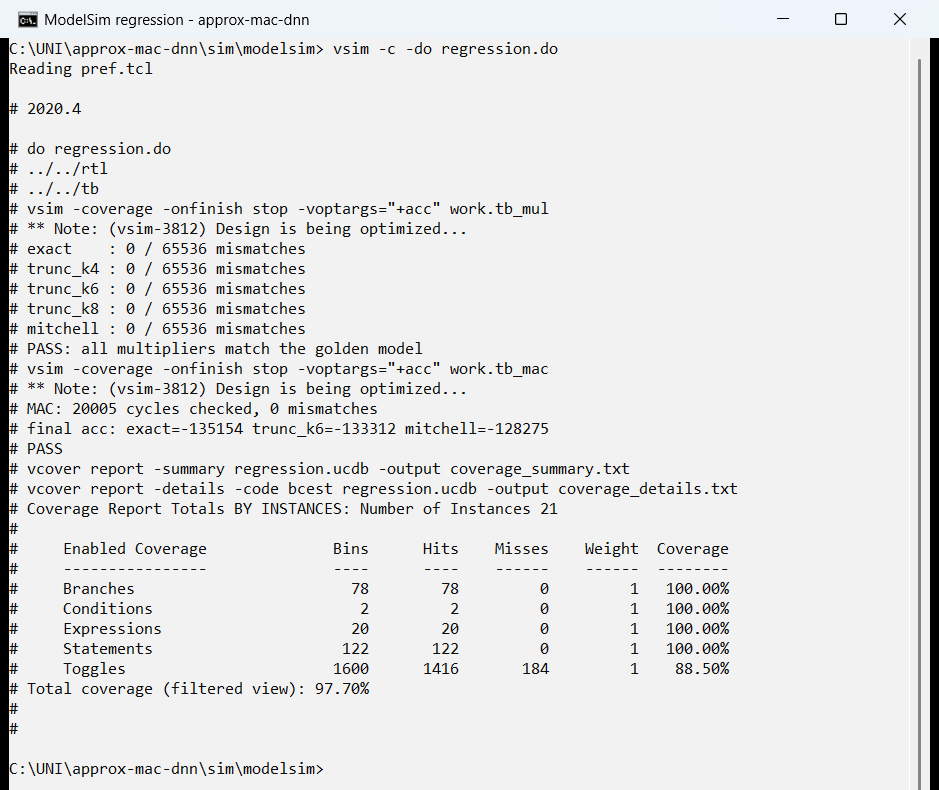
\includegraphics[width=0.78\textwidth]{modelsim_regression.png}
\caption{Batch regression in ModelSim (\texttt{vsim -c -do regression.do}):
exhaustive multiplier test, cycle-accurate MAC test and merged coverage
summary.}
\label{fig:msreg}
\end{figure}

\begin{table}[h]
\centering
\caption{Merged code coverage of the RTL over both testbenches (21 instances).}
\label{tab:cov}
\begin{tabular}{lrrr}
\toprule
Metric & Bins & Hit & Coverage (\%) \\
\midrule
Statements  & 122  & 122  & 100.0 \\
Branches    & 78   & 78   & 100.0 \\
Conditions  & 2    & 2    & 100.0 \\
Expressions & 20   & 20   & 100.0 \\
Toggles     & 1600 & 1416 & 88.5  \\
\bottomrule
\end{tabular}
\end{table}

All statements, branches, conditions and expressions are exercised
(Table~\ref{tab:cov}). Every missed toggle bin was inspected and is
structurally unreachable rather than a gap in the tests: the product bits
below column $K$ of the truncated multipliers are constant zero by design,
bit~15 of the product magnitude can never be set because the largest
magnitude is $128\times128=2^{14}$, and the upper bits of the 32-bit
accumulator are not reached by 784-term dot products of int8 data.

Figure~\ref{fig:msgui} shows the MAC test in the ModelSim GUI, opened with
\texttt{vsim -do gui.do}. The predefined layout (\texttt{wave\_mac.do})
groups the control signals, operands and, for each of the three MAC
variants, the RTL accumulator directly above the reference model, so that
any divergence is visible at a glance. The product of the operands applied
in one cycle appears in \texttt{p\_q} one cycle later and is added to
\texttt{acc} in the following cycle; while \texttt{en} is low the
accumulator holds its value. The \texttt{errs} counter stays at zero for
the whole run.

\begin{figure}[h]
\centering
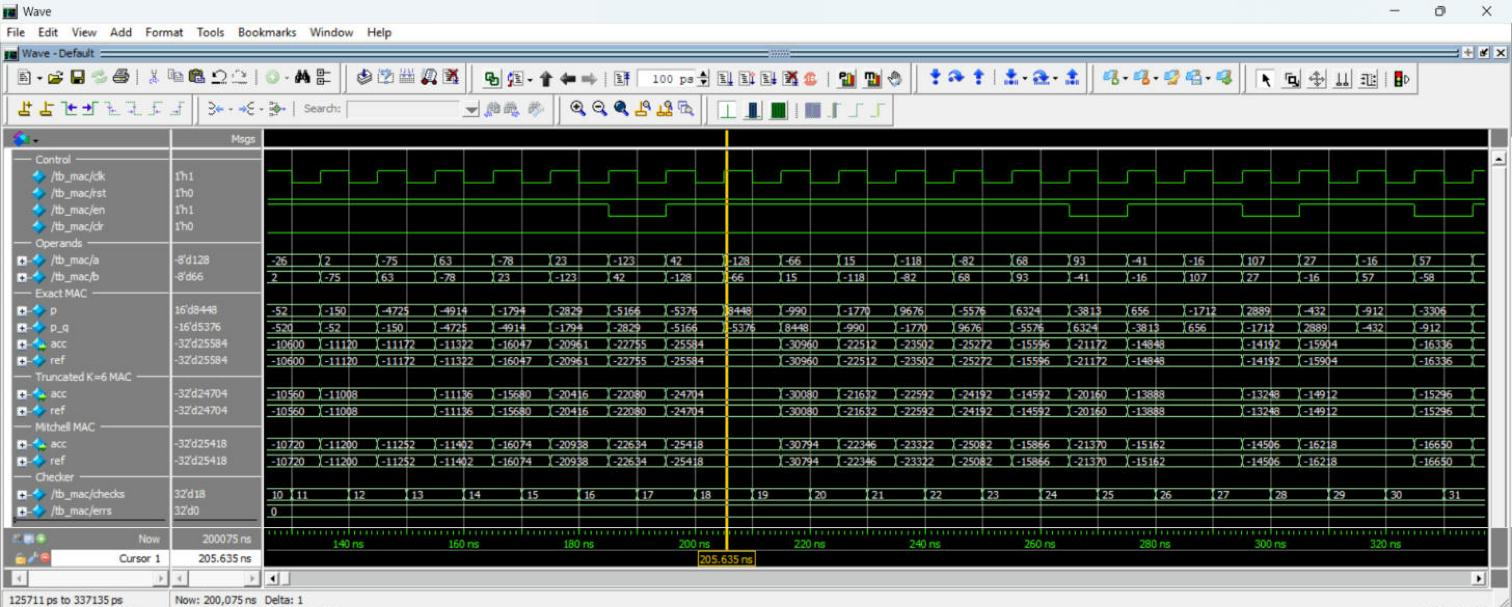
\includegraphics[width=\textwidth]{modelsim_wave.png}
\caption{ModelSim SE-64 2020.4 wave window during \texttt{tb\_mac}: exact,
truncated ($K=6$) and Mitchell MACs, each with its reference accumulator.}
\label{fig:msgui}
\end{figure}

\section{Logic Synthesis and Design-Space Exploration}
\label{sec:synth}

\subsection{Flow}
Each multiplier and MAC was synthesized with Yosys~0.70 and ABC
(\texttt{python/synth.py}). After flattening and generic optimization, the
netlist was mapped by ABC onto a technology-independent library of
2-input gates (AND, NAND, OR, NOR, XOR, XNOR, AND-NOT, OR-NOT) and 2:1
multiplexers. Area is reported in NAND2-equivalent gates (GE) using
relative cell areas typical of a standard-cell library (NAND2/NOR2 $=1$,
AND2/OR2 $=1.33$, XOR2/XNOR2/MUX2 $=2.33$, inverter $=0.67$, flip-flop
$\approx4.3$--$6$). Delay is approximated by the logic depth, i.e.\ the
number of gates on the longest combinational path. These figures are not
a substitute for a characterized PDK, but they are consistent across
designs and therefore suitable for relative comparison.

For every design the flow stores the complete Yosys log, including the
cell statistics and the longest path, and the gate-level netlist
(\texttt{results/synth/}). Figure~\ref{fig:yosysrun} shows a run of the
flow together with the statistics that Yosys reports for the truncated
multiplier with $K=8$; the 155 logic cells match Table~\ref{tab:synth}
(the additional \texttt{\$scopeinfo} entry is hierarchy metadata, not
logic). Figure~\ref{fig:schem} shows the MAC unit as elaborated by Yosys
before technology mapping: the multiplier instance, the pipeline
flip-flops (\texttt{\$dff}), the accumulator adder (\texttt{\$add}) and the
multiplexers implementing reset, enable and clear.

\begin{figure}[h]
\centering
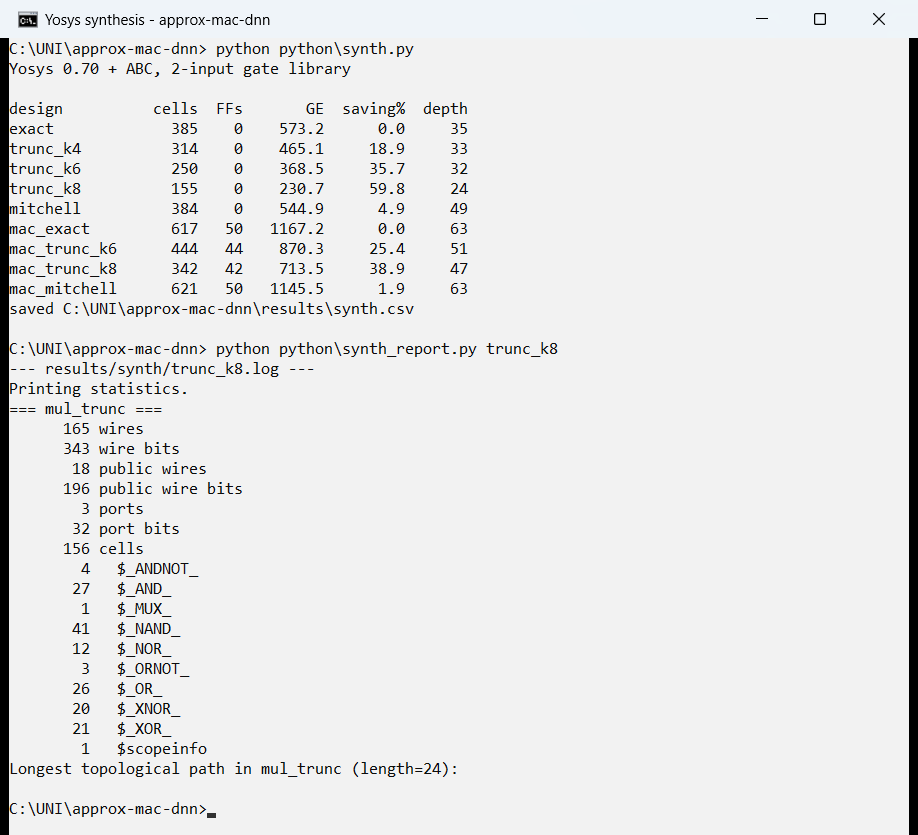
\includegraphics[width=0.72\textwidth]{synth/yosys_terminal.png}
\caption{Synthesis flow output and Yosys cell statistics of the truncated
multiplier ($K=8$), read from its synthesis log.}
\label{fig:yosysrun}
\end{figure}

\begin{figure}[h]
\centering
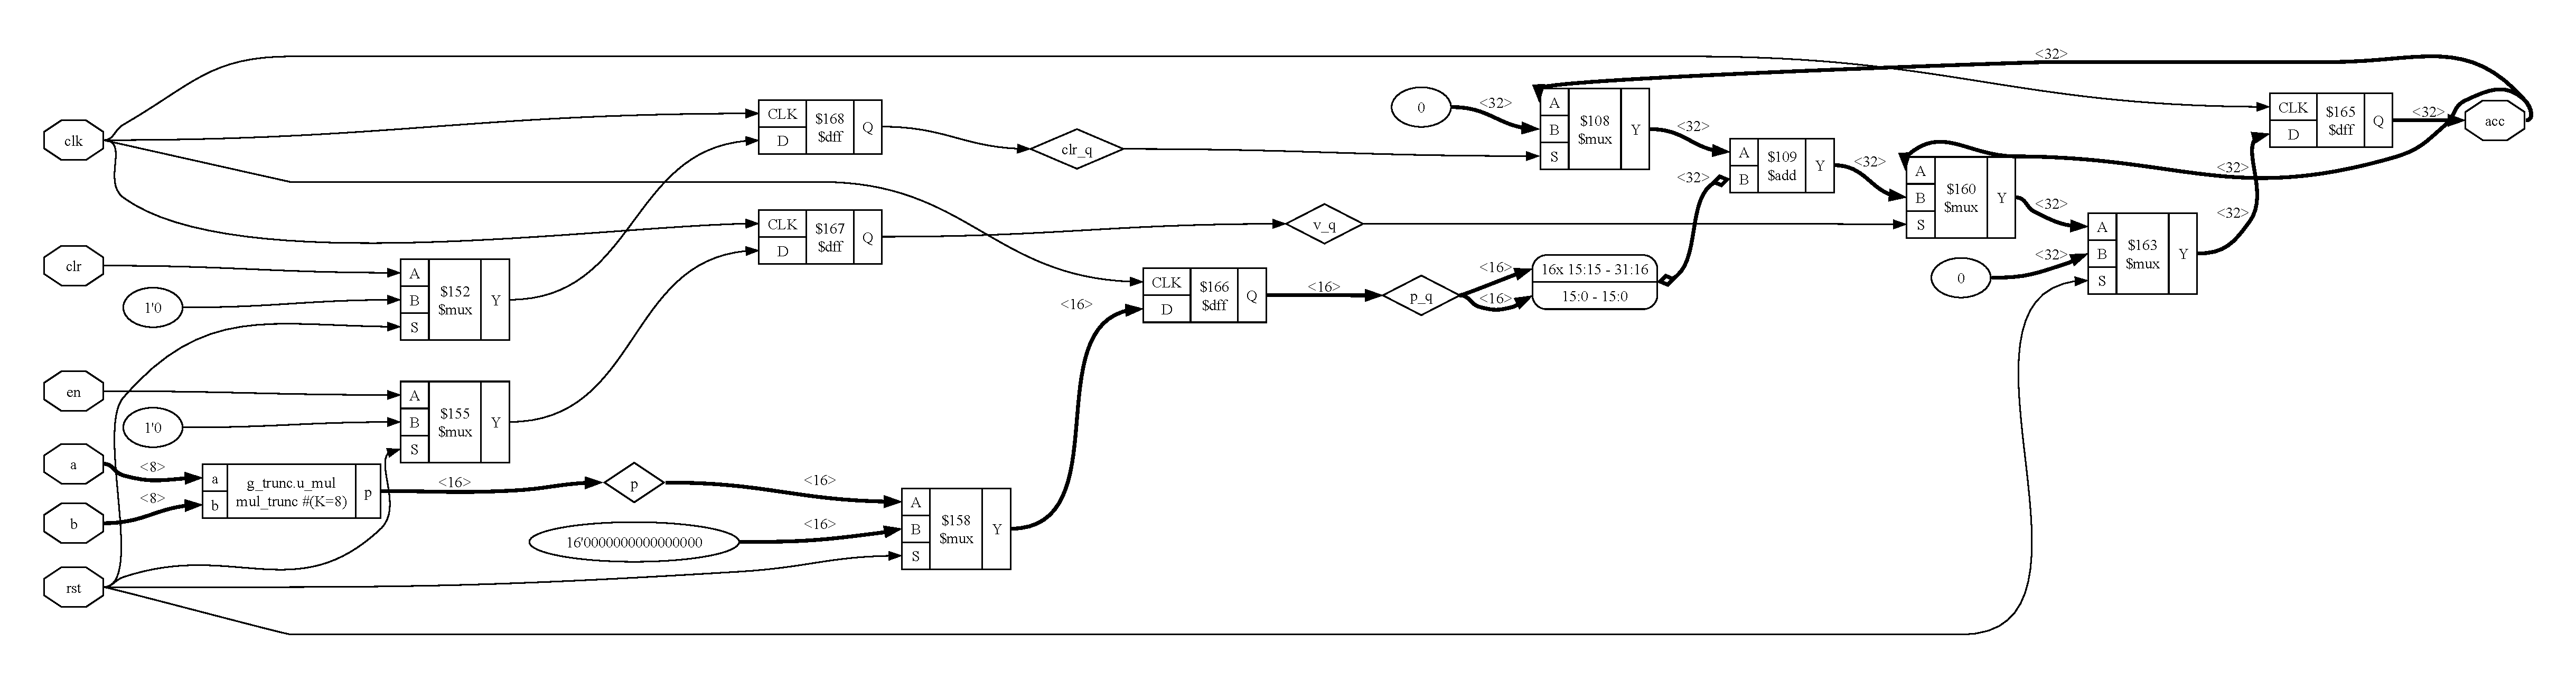
\includegraphics[width=\textwidth]{synth/mac_schematic.pdf}
\caption{Yosys schematic of the MAC unit with the truncated multiplier
($K=8$), generated with \texttt{show} after elaboration.}
\label{fig:schem}
\end{figure}

\subsection{Results}
\begin{table}[h]
\centering
\caption{Synthesis results. Savings are relative to the exact multiplier
or the exact MAC, respectively.}
\label{tab:synth}
\begin{tabular}{lrrrrr}
\toprule
Design & Cells & FFs & Area (GE) & Saving (\%) & Logic depth \\
\midrule
Exact multiplier   & 385 & 0  & 573.2  & --   & 35 \\
Truncated $K{=}4$  & 314 & 0  & 465.1  & 18.9 & 33 \\
Truncated $K{=}6$  & 250 & 0  & 368.5  & 35.7 & 32 \\
Truncated $K{=}8$  & 155 & 0  & 230.7  & 59.8 & 24 \\
Mitchell           & 384 & 0  & 544.9  & 4.9  & 49 \\
\midrule
MAC, exact         & 617 & 50 & 1167.2 & --   & 63 \\
MAC, trunc.\ $K{=}6$ & 444 & 44 & 870.3  & 25.4 & 51 \\
MAC, trunc.\ $K{=}8$ & 342 & 42 & 713.5  & 38.9 & 47 \\
MAC, Mitchell      & 621 & 50 & 1145.5 & 1.9  & 63 \\
\bottomrule
\end{tabular}
\end{table}

\begin{figure}[h]
\centering
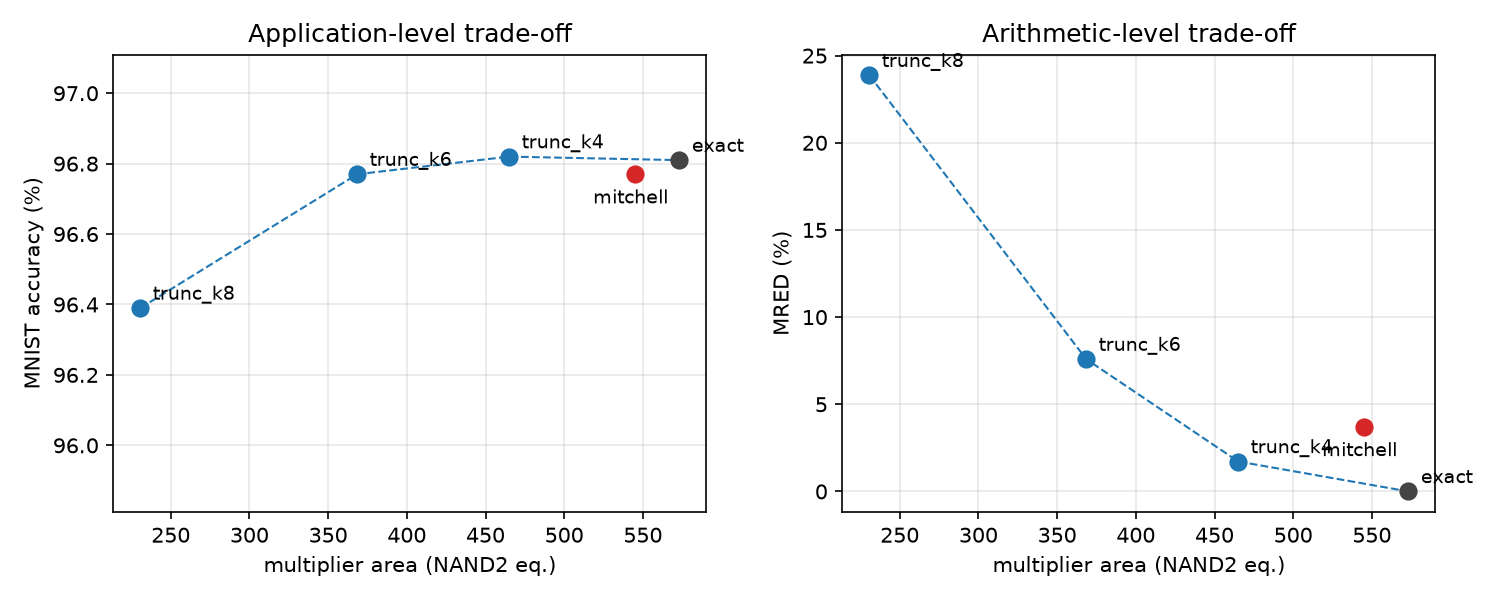
\includegraphics[width=\textwidth]{pareto.png}
\caption{Design space of the 8-bit multipliers. Left: MNIST accuracy versus
multiplier area. Right: mean relative error versus area. The dashed line
connects the truncation family.}
\label{fig:pareto}
\end{figure}

\subsection{Discussion}
\paragraph{Truncation dominates the design space.} Table~\ref{tab:synth}
and Figure~\ref{fig:pareto} show that column truncation provides an almost
linear area--error knob. Truncation at $K=6$ removes \SI{35.7}{\percent}
of the multiplier area for a \SI{0.04}{\percent} accuracy loss, and $K=8$
removes \SI{59.8}{\percent} for \SI{0.42}{\percent}. Truncation also
shortens the critical path, since the removed low-order columns shorten
the carry chain of the final adder. The saving carries over to the
complete PE: the MAC with $K=8$ is \SI{38.9}{\percent} smaller than the
exact MAC. Part of this comes for free, because the always-zero low bits
of the product are detected by synthesis and their pipeline flip-flops
are removed (50 $\rightarrow$ 42 FFs).

\paragraph{Mitchell is not efficient at 8 bits.} Although its error is
moderate (MRED \SI{3.7}{\percent}), the Mitchell multiplier saves only
\SI{4.9}{\percent} of the area and has the \emph{longest} critical path
(49 vs.\ 35 gates). Its overhead---two leading-one detectors, two barrel
shifters, a comparator and a final multiplexer---is roughly constant,
whereas the partial-product array it replaces grows quadratically with the
operand width. At 8 bits the array is still small, so the overhead
cancels most of the benefit. Logarithmic multipliers are therefore better
suited to wider datapaths (16 bits and above), while truncation-based
designs are preferable for int8 DNN accelerators. This is a
width-dependent conclusion that the error metrics alone would not reveal:
judged only by MRED, Mitchell appears better than truncation at $K=6$.

\paragraph{Error metrics do not predict accuracy.} Truncation at $K=6$
has twice the MRED of Mitchell but the same accuracy, and $K=8$ has
\SI{24}{\percent} MRED with less than half a point of accuracy loss.
Selecting approximate units for DNN accelerators therefore requires
application-level evaluation rather than arithmetic metrics alone.

\section{Conclusion}
\label{sec:next}
This work presented a complete evaluation flow for approximate arithmetic in
DNN accelerators, covering bit-accurate modelling, exhaustive RTL
verification, logic synthesis and quantized-network inference. For an int8
MLP on MNIST, a column-truncated multiplier with $K=8$ reduces multiplier
area by \SI{59.8}{\percent} and MAC area by \SI{38.9}{\percent} at a cost of
\SI{0.42}{\percent} in classification accuracy, and $K=6$ achieves a
\SI{35.7}{\percent} multiplier area reduction with no measurable accuracy
loss. The Mitchell logarithmic multiplier, despite a moderate arithmetic
error, offers less than \SI{5}{\percent} area reduction at this operand
width while lengthening the critical path. The results show that the
suitability of an approximate multiplier depends on the datapath width and
must be judged at the application level rather than by arithmetic error
metrics alone.

\section{Repository Structure}
\begin{lstlisting}
python/approx_mult.py       bit-accurate multiplier models
python/error_analysis.py    exhaustive error metrics and heatmaps
python/train_quantize.py    NumPy MLP training and int8 quantization
python/approx_inference.py  inference through approximate multipliers
python/gen_vectors.py       golden vectors for RTL verification
python/synth.py             Yosys/ABC synthesis, area and logic depth
python/synth_report.py      cell statistics from a synthesis log
python/pareto.py            design-space plot and summary table
docs/figures/mac_unit.tex   MAC block diagram (TikZ)
rtl/                        Verilog: sign_mag, mul_exact, mul_trunc,
                            mul_mitchell, mac
tb/                         self-checking testbenches, run_sim.sh
sim/modelsim/               ModelSim project, do-scripts, coverage flow
results/                    metrics (CSV), figures, quantized model
docs/report.tex             this report
\end{lstlisting}
All experiments are reproducible with
\texttt{pip install -r requirements.txt}, running the Python scripts in the
order listed above, and \texttt{vsim -c -do regression.do} in
\texttt{sim/modelsim} for the RTL regression with coverage
(\texttt{sh tb/run\_sim.sh} provides a minimal flow that also works with
Icarus Verilog).

\begin{thebibliography}{9}
\bibitem{mitchell1962}
J.~N. Mitchell, ``Computer multiplication and division using binary
logarithms,'' \emph{IRE Transactions on Electronic Computers}, vol.~EC-11,
no.~4, pp.~512--517, 1962.

\bibitem{jiang2020survey}
H.~Jiang, F.~J.~H. Santiago, H.~Mo, L.~Liu, and J.~Han, ``Approximate
arithmetic circuits: A survey, characterization, and recent applications,''
\emph{Proceedings of the IEEE}, vol.~108, no.~12, pp.~2108--2135, 2020.

\bibitem{mrazek2017}
V.~Mrazek, R.~Hrbacek, Z.~Vasicek, and L.~Sekanina, ``EvoApprox8b: Library of
approximate adders and multipliers for circuit design and benchmarking of
approximation methods,'' in \emph{Proc.\ DATE}, 2017, pp.~258--261.

\bibitem{jacob2018}
B.~Jacob \emph{et al.}, ``Quantization and training of neural networks for
efficient integer-arithmetic-only inference,'' in \emph{Proc.\ CVPR}, 2018,
pp.~2704--2713.

\bibitem{lecun1998}
Y.~LeCun, L.~Bottou, Y.~Bengio, and P.~Haffner, ``Gradient-based learning
applied to document recognition,'' \emph{Proceedings of the IEEE}, vol.~86,
no.~11, pp.~2278--2324, 1998.
\end{thebibliography}

\end{document}
